\documentclass[a4]{article}
\pagestyle{myheadings}

%%%%%%%%%%%%%%%%%%%
% Packages/Macros %
%%%%%%%%%%%%%%%%%%%
\usepackage{mathrsfs}


\usepackage{fancyhdr}
\pagestyle{fancy}
\lhead{}
\chead{}
\rhead{}
\lfoot{}
\cfoot{} 
\rfoot{\normalsize\thepage}
\renewcommand{\headrulewidth}{0pt}
\renewcommand{\footrulewidth}{0pt}
\newcommand{\RomanNumeralCaps}[1]
    {\MakeUppercase{\romannumeral #1}}

\usepackage{amssymb,latexsym}  % Standard packages
\usepackage[utf8]{inputenc}
\usepackage[russian]{babel}
\usepackage{MnSymbol}
\usepackage{mathrsfs}
\usepackage{amsmath,amsthm}
\usepackage{indentfirst}
\usepackage{graphicx}%,vmargin}
\usepackage{graphicx}
\graphicspath{{pictures/}} 
\usepackage{verbatim}
\usepackage{color}
\usepackage{color,colortbl}
\usepackage[nottoc,numbib]{tocbibind}
\usepackage{float}
\usepackage{multirow}
\usepackage{hhline}

\usepackage{listings}
\definecolor{codegreen}{rgb}{0,0.6,0}
\definecolor{codegray}{rgb}{1,1,1}
\definecolor{codepurple}{rgb}{0.58,0,0.82}
\definecolor{backcolour}{rgb}{0.95,0.95,0.92}
 
\lstdefinestyle{mystyle}{
    backgroundcolor=\color{backcolour},   
    commentstyle=\color{codegreen},
    keywordstyle=\color{magenta},
    numberstyle=\tiny\color{codegray},
    stringstyle=\color{codepurple},
    basicstyle=\footnotesize,
    breakatwhitespace=false,         
    breaklines=true,                 
    captionpos=b,                    
    keepspaces=true,                 
    numbers=left,                    
    numbersep=5pt,                  
    showspaces=false,                
    showstringspaces=false,
    showtabs=false,                  
    tabsize=2
}
 
\lstset{style=mystyle}

\usepackage{url}
\urldef\myurl\url{foo%.com}
\def\UrlBreaks{\do\/\do-}
\usepackage{breakurl}
\Urlmuskip=0mu plus 1mu



\DeclareGraphicsExtensions{.pdf,.png,.jpg}% -- настройка картинок

\usepackage{epigraph} %%% to make inspirational quotes.
\usepackage[all]{xy} %for XyPic'a
\usepackage{color} 
\usepackage{amscd} %для коммутативных диграмм
%\usepackage[colorlinks,urlcolor=red]{hyperref}

%\renewcommand{\baselinestretch}{1.5}
%\sloppy
%\usepackage{listings}
%\lstset{numbers=left}
%\setmarginsrb{2cm}{1.5cm}{1cm}{1.5cm}{0pt}{0mm}{0pt}{13mm}


\newtheorem{Lemma}{Лемма}[section]
\newtheorem{Proposition}{Предложение}[section]
\newtheorem{Theorem}{Теорема}[section]
\newtheorem{Corollary}{Следствие}[section]
\newtheorem{Remark}{Замечание}[section]
\newtheorem{Definition}{Определение}[section]
\newtheorem{Designations}{Обозначение}[section]




%%%%%%%%%%%%%%%%%%%%%%% 
%Подготовка оглавления% 
%%%%%%%%%%%%%%%%%%%%%%% 
\usepackage[titles]{tocloft}
\renewcommand{\cftdotsep}{2} %частота точек
\renewcommand\cftsecleader{\cftdotfill{\cftdotsep}}
\renewcommand{\cfttoctitlefont}{\hspace{0.38\textwidth} \LARGE\bfseries} 
\renewcommand{\cftsecaftersnum}{.}
\renewcommand{\cftsubsecaftersnum}{.}
\renewcommand{\cftbeforetoctitleskip}{-1em} 
\renewcommand{\cftaftertoctitle}{\mbox{}\hfill \\ \mbox{}\hfill{\footnotesize Стр.}\vspace{-0.5em}} 
%\renewcommand{\cftchapfont}{\normalsize\bfseries \MakeUppercase{\chaptername} } 
%\renewcommand{\cftsecfont}{\hspace{1pt}} 
\renewcommand{\cftsubsecfont}{\hspace{1pt}} 
%\renewcommand{\cftbeforechapskip}{1em} 
\renewcommand{\cftparskip}{3mm} %определяет величину отступа в оглавлении
\setcounter{tocdepth}{5} 
\renewcommand{\listoffigures}{\begingroup %добавляем номер в список иллюстраций
\tocsection
\tocfile{\listfigurename}{lof}
\endgroup}
\renewcommand{\listoftables}{\begingroup %добавляем номер в список иллюстраций
\tocsection
\tocfile{\listtablename}{lot}
\endgroup}


%\renewcommand{\thelikesection}{(\roman{likesection})}
%%%%%%%%%%%
% Margins %
%%%%%%%%%%%
\addtolength{\textwidth}{0.7in}
\textheight=630pt
\addtolength{\evensidemargin}{-0.4in}
\addtolength{\oddsidemargin}{-0.4in}
\addtolength{\topmargin}{-0.4in}

%%%%%%%%%%%%%%%%%%%%%%%%%%%%%%%%%%%
%%%%%%Переопределение chapter%%%%%% 
%%%%%%%%%%%%%%%%%%%%%%%%%%%%%%%%%%%
\newcommand{\empline}{\mbox{}\newline} 
\newcommand{\likechapterheading}[1]{ 
\begin{center} 
\textbf{\MakeUppercase{#1}} 
\end{center} 
\empline} 

%%%%%%%Запиливание переопределённого chapter в оглавление%%%%%% 
\makeatletter 
\renewcommand{\@dotsep}{2} 
\newcommand{\l@likechapter}[2]{{\bfseries\@dottedtocline{0}{0pt}{0pt}{#1}{#2}}} 
\makeatother 
\newcommand{\likechapter}[1]{ 
\likechapterheading{#1} 
\addcontentsline{toc}{likechapter}{\MakeUppercase{#1}}} 




\usepackage{xcolor}
\usepackage{hyperref}
\definecolor{linkcolor}{HTML}{000000} % цвет ссылок
\definecolor{urlcolor}{HTML}{AA1622} % цвет гиперссылок
 
\hypersetup{pdfstartview=FitH,  linkcolor=linkcolor,urlcolor=urlcolor, colorlinks=true}

%%%%%%%%%%%%
% Document %
%%%%%%%%%%%%

%%%%%%%%%%%%%%%%%%%%%%%%%%%%%
%%%%%%главы -- section*%%%%%%
%%%%section -- subsection%%%%
%subsection -- subsubsection%
%%%%%%%%%%%%%%%%%%%%%%%%%%%%%
\def \newstr {\medskip \par \noindent} 



\begin{document}
\def\contentsname{\LARGE{Содержание}}
\thispagestyle{empty}
\begin{center} 

\vspace{2cm} 
{\Large \sc Санкт-Петербургский Политехнический}\\
\vspace{2mm}
{\Large \sc Университет} им. {\Large\sc Петра Великого}\\
\vspace{1cm}
{\large \sc Институт прикладной математики и механики\\ 
\vspace{0.5mm}
\textsc{}}\\ 
\vspace{0.5mm}
{\large\sc Кафедра прикладной математики}\\
\vspace{15mm}


%\rule[0.5ex]{\linewidth}{2pt}\vspace*{-\baselineskip}\vspace*{3.2pt} 
%\rule[0.5ex]{\linewidth}{1pt}\\[\baselineskip] 
{\huge \sc Сводный отчет по лабораторным 5-8.

 }
\vspace*{2mm}
%\rule[0.7ex]{\linewidth}{1pt}\vspace*{-\baselineskip}\vspace{3.2pt} 
%\rule[0.5ex]{\linewidth}{2pt}\\ 


\vspace{1cm}

{\sc $3$ курс$,$ группа $3630102/70301$}

\vspace{2cm} 
Студент группы $3630102/70301$ \hfill Лебедев К.С.\\
\vspace{1cm}
Преподаватель \hfill Баженов А. Н.\\
\vspace{20mm} 

\end{center} 
%\author{Я}
\begin{center}
\vfill {\large\textsc{Санкт-Петербург}}\\ 
2020 г.
\end{center}

%%%%%%%%%%%%%%%%%%%%%%%%%%%%%%%%%%%%%%%%%%%%%%%%%%%%%%%%%%%%%%%%%%%%%%%%%%%%%%%%%%%%%%%%%%%%%%
%\ \\[4cm]

%\rm
%%%%%%%%%%%%%%%%%%%%%%%%%%%%%%%%%%%%%%%%%%%%%%%%%%%%%%%%%%%%%%%%%%%%%%%%%%%%%%%%%%%%%%%%%%%%%%
\newpage
\pagestyle{plain}

%\begin{center}
%\begin{abstract} 

%\end{abstract}

%\end{center}

\newpage
\tableofcontents{}
\newpage
\listoffigures{}
\newpage

\section{Постановка задачи}
\begin{enumerate}
	\item Построить выборки для двумерного нормального распределения с коэффициентами корреляции $\rho = 0, 0.5, 0.9$. Вычислить коэффициент корреляции Пирсона, Спирмана и квадрантный коэффициент корреляции для каждой выборки. 
	Повторить вычисления для смеси двумерных нормальных распределений: 
	\begin{equation}
	    f(x,y) = 0.9N(x,y,0,0,1,1,0.9)+0.1N(x,y,0,0,10,10,-0.9)
	\end{equation}
	\item Найти оценки линейной регрессии $y_i=a+bx_i+e_i,$ используя $20$ точек отрезка $[-1.8;\;2]$ с равномерным шагом. Ошибку $e_i$ считать нормально распределённой с параметрами $(0,\;1).$ В качестве эталонной зависимости взять $y_i=2+2x_i+e_i.$ При построении оценок коэффициентов использовать два критерия: 
	\begin{itemize}
	\item Критерий наименьших квадратов 
	\item Критерий наименьших модулей
	\end{itemize}
	Проделать то же самое для выборки, у которой в значении $y_1$ и $y_{20}$ вносятся возмущения $10$ и $-10$ соответственно.
	\item Cгенерировать выборку объемом $100$ элементов для нормального распределения $N(x;0,1).$ По сгенерированной выборке оценить параметры $\mu$ и $\sigma$ нормального закона методом максимального правдоподобия. В качестве основной гипотезы $H_0$ будем считать, что сгенерированное распределение имеет вид $N(x,\overset{\wedge}{\mu},\overset{\wedge}{\sigma} ).$ Проверить основную гипотезу, используя критерий согласия $\chi$.
	\item Для двух выборок $20$ и $100$ элементов, сгенерированных согласно нормальному закону $N(x,0,1),$ для параметров масштаба и положения построить асимптотически нормальные интервальные оценки на основе точечных оценок метода максимального правдоподобия и классические интервальные оценки на основе статистик $\chi^2$ и Стьюдента.
	\end{enumerate}
	\section{Теория} % (fold)
	\subsection{Вычисление коэффициента корреляции} % (fold)
	\label{sub:вычисление_коэффициента_корреляции}
	\begin{enumerate}
	    \item Двумерное нормально распределение \cite{5_1}:
	        \begin{equation}
	        N(x,y,0,0,1,1,\rho) = \frac{1}{2\pi\sqrt{1-\rho^2}}e^{-\frac{1}{2(1-\rho^2)}(x^2-2\rho x y+y^2)} \label{dnd}
	        \end{equation}
	    
	    \item Коэффициент корреляции Пирсона \cite{5_2}:
	        \begin{equation}
	        r_{xy} = \left(\sum\limits_{i=1}^n(x_i-\overline{x})(y_i-\overline{y})\right)\left(\sum\limits_{i=1}^n(x_i-\overline{x})^2\sum\limits_{i=1}^n(y_i-\overline{y})^2\right)^{-\frac{1}{2}} \label{ccp}
	        \end{equation}
	    \item Коэффициент корреляции Спирмана \cite{5_3}:
	        \begin{equation}
	        \rho_n = 1 -  \frac{6}{n^3-n}\sum\limits_{i=1}^n d_i^2\label{ccs}
	        \end{equation}
	        
	    \item Квадрантный коэффициент корреляции \cite{5_4}:
	        \begin{equation}
	        \overset{\wedge}{q} = \frac{1}{n}\sum\limits_{i=1}^n sign(x_i-med\;x)sign(y_i-med\;y)\label{qcc}
	        \end{equation}
	\end{enumerate}
	% subsection вычисление_коэффициента_корреляции (end)
	% section  (end)
	\subsection{Оценка регрессии} % (fold)
	\label{sub:оценка_регрессии}
	Простая линейная регрессия \cite{lin_reg}:
	\begin{equation}
	    y_i=ax_i+b+e_i,\;i=\overline{1,n},\hfill
	\end{equation}

	где $x_i\;\--$ заданные числа, $y_i\;\--$ наблюдаемые значения, $e_i\;\--$ независимы и нормально распределены, $a$ и $b\;\--$ неизвестные параметры, подлежащие оцениванию.

	\begin{enumerate}
	\item \textit{Метод наименьших квадратов}\\
	Критерий $\--$ минимизация функции:
	\begin{equation}
	    Q(a,b)=\sum\limits_{i=1}^n(y_i-ax_i-b)^2\to \min\hfill
	\end{equation}

	Оценка $\overset{\wedge}{a}$ и $\overset{\wedge}{b}$ параметров $a$ и $b,$ в которых достигается минимум $Q(a,b),$ называются МНК-оценками. В случае линейной регрессии их можно вычислить из формулы :
	\begin{equation}
	    \begin{cases}
	    \overset{\wedge}{a} = \frac{\overline{x y}-\overline{x}\overline{y}}{\overline{x^2}-\overline{x}^2}\\
	    \overset{\wedge}{b} = \overline{y}-\overset{\wedge}{a}\overline{x}
	    \end{cases}\hfill
	\end{equation}

	Метод наименьших квадратов является несмещённой оценкой.


	\item \textit{Метод наименьших модулей}\\
	Критерий наименьших модулей – заключается в минимизации следующей функции :
	\begin{equation}
	    M(a,b) = \sum\limits_{i=1}^n\vert y_i-ax_i-b\vert\to\min\hfill
	\end{equation}

	МНМ-оценки обладают свойством робастности
	\end{enumerate}
	% subsection оценка_регрессии (end)
	\subsection{Точечная оценка параметров распределения} % (fold)
		\label{sub:точечная_оценка_параметров_распределения}
	\begin{enumerate}
			\item \textit{Метод максимального правдоподобия}\\
	Метод максимального правдоподобия $\--$ метод оценивания неизвестного параметра путём максимизации функции правдоподобия.
	\begin{equation}
	    \overset{\wedge}{\theta}_{\text{МП}}=argmax \mathbf{L}(x_1,x_2,\ldots,x_n,\theta)
	\end{equation}

	Где $\mathbf{L}$ это функция правдоподобия, которая представляет собой совместную плотность вероятности независимых случайных величин $X_1,x_2,\ldots,x_n$ и является функцией неизвестного параметра $\theta$
	\begin{equation}
	    \mathbf{L} = f(x_1,\theta)\cdot f(x_2,\theta)\cdot\cdots\cdot f(x_n,\theta)
	\end{equation}
	Оценкой максимального правдоподобия будем называть такое значение $\overset{\wedge}{\theta}_{\text{МП}}$ из множества допустимых значений параметра $\theta,$ для которого функция правдоподобия принимает максимальное значение при заданных $x_1,x_2,\ldots,x_n.$

	Тогда при оценивании математического ожидания $m$ и дисперсии $\sigma^2$ нормального распределения $N(m,\sigma)$ получим:
	\begin{equation}
	    \ln(\mathbf{L})=-\frac{n}{2}\ln(2\pi)-\frac{n}{2}\ln\left(\sigma^2\right)-\frac{1}{2\sigma^2}\sum\limits_{i=1}^n(x_i-m)^2
	\end{equation}
	\item \textit{Критерий согласия Пирсона}\\
	Разобьём генеральную совокупность на $k$ непересекающихся подмножеств $\Delta_1, \Delta_2,\ldots, \Delta_k,\;\Delta_i = (a_i,a_{i+1}],$ $p_i = P(X\in\Delta_i),\;i=1,2,\ldots,k\; \--$ вероятность того, что точка попала в $i$ый промежуток.

	Так как генеральная совокупность это $\mathbb{R},$ то крайние промежутки будут бесконечными: $\Delta_1=(-\infty,a_1],\;\Delta_k=(a_k,\infty),\;p_i = F(a_i)-F(a_{i-1})$

	$n_i\;\--$ частота попадания выборочных элементов в $\Delta_i,\;i=1,2,\ldots,k.$

	В случае справедливости гипотезы $H_0$ относительно частоты $\frac{n_i}{n}$ при больших $n$ должны быть близки к $p_i,$ значит в качестве меры имеет смысл взять: 
	\begin{equation}
	    Z = \sum\limits_{i=1}^k\frac{n}{p_i}\left(\frac{n_i}{n}-p_i\right)^2
	\end{equation}
	Тогда
	\begin{equation}
	    \chi^2_B=\sum\limits_{i=1}^k\frac{n}{p_i}\left(\frac{n_i}{n}-p_i\right)^2=\sum\limits_{i=1}^k\frac{(n_i-np_i)^2}{np_i}
	\end{equation}
	Для выполнения гипотезы $H_0$ должны выполняться следующие условия :
	\begin{equation}
	    \chi_B^2 < \chi_{1-\alpha}^2(k-1)
	\end{equation}
	где $\chi_{1-\alpha}^2(k-1)\;\--$ квантиль распределения $\chi^2$ с $k-1$ степенями свободы порядка $1-\alpha,$ где $\alpha$ заданный уровень значимости.
		\end{enumerate}	
		% subsection точечная_оценка_параметров_распределения (end)	
	\subsection{Интервальные оценки} % (fold)
	\label{sub:интервальные_оценки}
	Оценкой максимального правдоподобия для математического ожидания  является среднее арифметическое: $\mu=\frac{1}{n}\sum\limits_{i=1}^nx_i.$

	Оценка максимального правдоподобия для дисперсии вычисляется по формуле: $\sigma^2 = \frac{1}{n}\sum\limits_{i=1}^n(x_i-\overline{x})^2.$

	Доверительным интервалом или интервальной оценкой числовой характеристики или параметра распределения $\theta$ с доверительной вероятностью $\gamma$ называется интервал со случайными границами $(\theta_1,\theta_2),$ содержащий параметр $\theta$ с вероятностью $\gamma$ \cite{8_1}.

	Функция распределения Стьюдента :
	\begin{equation}
	    T = \sqrt{n-1}\frac{\overline{x}-\mu}{\delta}
	\end{equation}

	Функция плотности распределения $\chi^2$ :
	\begin{equation}
	    f(x) = \begin{cases}
	    0,&x\leq 0\\
	    \frac{1}{2^\frac{n}{2}\Gamma\left(\frac{n}{2}\right)}x^{\frac{n}{2}-1}e^{-\frac{x}{2}},& x>0
	    \end{cases}
	\end{equation}

	Интервальная оценка математического ожидания :
	\begin{equation}
	    P=\left(\overline{x}-\frac{\sigma t_{1-\frac{a}{2}}(n-1)}{\sqrt{n-1}}<\mu<\overline{x}+\frac{\sigma t_{1-\frac{a}{2}}(n-1)}{\sqrt{n-1}}\right) = \gamma,
	\end{equation}
	где $t_{1-\frac{a}{2}}\;\--$ квантиль распределения Стьюдента порядка $1-\frac{a}{2}.$

	Интервальная оценка дисперсии:
	\begin{equation}
	    P=\left(\frac{\sigma\sqrt{n}}{\sqrt{\chi^2_{1-\frac{a}{2}}(n-1)}}<\sigma<\frac{\sigma\sqrt{n}}{\sqrt{\chi^2_\frac{a}{2}(n-1)}}\right) = \gamma,
	\end{equation}
	где $\chi_{1-\frac{a}{2}}^2,\;\chi_\frac{a}{2}^2\;\--$ квантили распределения Стьюдента порядков $1-\frac{a}{2}$ и $\frac{a}{2}$ соответственно.

	Асимптотическая интервальная оценка математического ожидания :
	\begin{equation}
	    P = \left(\overline{x}-\frac{\sigma u_{1-\frac{a}{2}}}{\sqrt{n}}<\mu<\overline{x}+\frac{\sigma u_{1-\frac{a}{2}}}{\sqrt{n}}\right)=\gamma,
	\end{equation}
	где $u_{1-\frac{a}{2}}\;\--$ квантиль нормального распределения $N(x,0,1)$ порядка $1-\frac{a}{2}.$
	% subsection интервальные_оценки (end)
	\section{Реализация} % (fold)
	\label{sec:реализация}
	Работы была выполнена на языке $Python 3.6.$
	Для генерации выборок использовался модуль \cite{numpy}.
	Для построения графиков использовалась библиотека matplotlib \cite{plotlib}.
	Функции распределения обрабатывались при помощи библиотеки scipy.stats \cite{skp}
	% section реализация (end)
\section{Результаты} % (fold)
\label{sec:результаты}
\subsection{Вычисление коэффицентов кореляции} % (fold)
\label{sub:вычисление_коэффицентов_кореляции}
\begin{figure}[H]
    \centering
    \caption{Графики двумерного нормального распределения\eqref{dnd} при $p=0.0$ }
    \includegraphics[scale = 0.8]{lab5/Figure_0.png} 
    \label{fig:dis_norm_gis0}
\end{figure}
\begin{table}[H]
\caption{Результаты для двумерного нормального распределения \eqref{dnd} при $p=0.0$}
\label{tab:my_label1}
\begin{center}
\vspace{5mm}
\begin{tabular}{|c|c|c|c|c|c|c|c|c|}
\hhline{----~----}
\multicolumn{4}{|c|}{Normal  $n=20,\;  p=0.0$} &\multirow{11}{*}{$\cdot$} & \multicolumn{4}{c|} {Normal  $n=60,\;  p=0.0$}
\\
\hhline{----~----}
&Pearson     &Spearman    &Quad &   & & Pearson     &Spearman    &Quad        \\    
\hhline{----~----}
		E   &$0.09570$&0.04511&-0.06000&  &E   &0.01801&0.01759&-0.00000\\
\hhline{----~----}
		$E^2$ &0.11247&0.094586&0.06800&  &$E^2$ &0.01451&0.01401&0.01422\\
\hhline{----~----}
		D   &0.10331&0.09255&0.06440&  &D   &0.01419&0.01370&0.01422\\\rowcolor{codegray}
\hhline{----~----} 
\multicolumn{9}{c}{}\\
\hhline{----~----}
\multicolumn{4}{|c|}{Normal  $n=100,\;  p=0.0$} & & \multicolumn{4}{c|}{Normal  $n=1000,\;  p=0.0$}\\
\hhline{----~----}
&Pearson     &Spearman    &Quad&  & &Pearson     &Spearman    &Quad     \\
\hhline{----~----}
		E   &0.07958&0.07688&0.09200& &E   &-0.01074&	-0.00817&	-0.00800\\
\hhline{----~----}
		$E^2$ &0.01358&	0.01452&	0.01680& &$E^2$ &0.00080&	0.00082&	0.00096\\
\hhline{----~----}
		D   &0.00725&	0.00861&	0.00834& &D   &0.00069	&0.00075	&0.00090\\
\hhline{----~----}
\end{tabular}
\end{center}
\end{table}




\vspace{-10cm}
\begin{figure}[H]
    \centering
    \caption{Графики двумерного нормального распределения\eqref{dnd} при $p=0.5$ }
    \includegraphics{lab5/Figure_1.png}
    \label{fig:dis_norm_gis1}
\end{figure}
\begin{table}[H]
\caption{Результаты для двумерного нормального распределения \eqref{dnd} при $p=0.5$}
\label{tab:my_label2}
\begin{center}
\vspace{5mm}
\begin{tabular}{|c|c|c|c|c|c|c|c|c|}
\hhline{----~----}
\multicolumn{4}{|c|}{Normal  $n=20,\;  p=0.5$} &\multirow{11}{*}{$\cdot$} & \multicolumn{4}{c|} {Normal  $n=60,\;  p=0.5$}
\\
\hhline{----~----}
&Pearson     &Spearman    &Quad &   & & Pearson     &Spearman    &Quad        \\    
\hhline{----~----}
		E   &0.56562&0.53910&0.28000&  &E   &0.44858&	0.44378&	0.28667\\
\hhline{----~----}
		$E^2$ &0.32763&	0.29964	&0.12800&  &$E^2$ &0.20459&	0.20291&	0.10356\\
\hhline{----~----}
		D   &0.00770	&0.00901	&0.04960&  &D   &0.00336&	0.00597&	0.02138\\\rowcolor{codegray}
\hhline{----~----} 
\multicolumn{9}{c}{}\\
\hhline{----~----}
\multicolumn{4}{|c|}{Normal  $n=100,\;  p=0.5$} & & \multicolumn{4}{c|}{Normal  $n=1000,\;  p=0.5$}\\
\hhline{----~----}
&Pearson     &Spearman    &Quad&  & &Pearson     &Spearman    &Quad     \\
\hhline{----~----}
		E   &0.50044&	0.49137&	0.31600& &E   &0.49722	&0.48120	&0.32320\\
\hhline{----~----}
		$E^2$ &0.25552&	0.24642&	0.10960& &$E^2$ &0.24757	&0.23175&	0.10468\\
\hhline{----~----}
		D   &0.00509&	0.00497&	0.00974& &D   &0.00034&	0.00020&	0.00022\\
\hhline{----~----}
\end{tabular}
\end{center}
\end{table}



\vspace{-1cm}
\begin{figure}[H]
    \centering
    \caption{График двумерного нормального распределения \eqref{dnd} при $p=0.9$ }
    \includegraphics{lab5/Figure_2.png} 
    \label{fig:dis_norm_gis2}
\end{figure}
\begin{table}[H]
\caption{Результаты для двумерного нормального распределения \eqref{dnd} при $p=0.9$}
\label{tab:my_label3}
\begin{center}
\vspace{5mm}
\begin{tabular}{|c|c|c|c|c|c|c|c|c|}
\hhline{----~----}
\multicolumn{4}{|c|}{Normal  $n=20,\;  p=0.9$} &\multirow{11}{*}{$\cdot$} & \multicolumn{4}{c|} {Normal  $n=60,\;  p=0.9$}
\\
\hhline{----~----}
&Pearson     &Spearman    &Quad &   & & Pearson     &Spearman    &Quad        \\    
\hhline{----~----}
		E   &0.90608&	0.88421&	0.76000&  &E   &0.89748&	0.87538	&0.68667\\
\hhline{----~----}
		$E^2$ &0.82263&	0.78440&	0.58400&  &$E^2$ &0.80573&	0.76683&	0.48844\\
\hhline{----~----}
		D   &0.00165	&0.00257&	0.00640&  &D   &0.00027&	0.00054	&0.01693\\\rowcolor{codegray}
\hhline{----~----} 
\multicolumn{9}{c}{}\\
\hhline{----~----}
\multicolumn{4}{|c|}{Normal  $n=100,\;  p=0.9$} & & \multicolumn{4}{c|}{Normal  $n=1000,\;  p=0.9$}\\
\hhline{----~----}
&Pearson     &Spearman    &Quad&  & &Pearson     &Spearman    &Quad     \\
\hhline{----~----}
		E   &0.88816&	0.87734&	0.70000& &E   &0.90323&	0.89562&	0.71400\\
\hhline{----~----}
		$E^2$ &0.78938&	0.77048&	0.49680& &$E^2$ &0.81584&	0.80215&	0.50995\\
\hhline{----~----}
		D   &0.00055&	0.00076&	0.00680& &D   &0.00001&	0.00001	&0.00015\\
\hhline{----~----}
\end{tabular}
\end{center}
\end{table}





\vspace{-1cm}
\begin{figure}[H]
    \centering
    \caption{Графики смеси двумерных нормальных распределений }
    \includegraphics{lab5/Figure_3.png} 
    \label{fig:dis_norm_gis4}
\end{figure}
\begin{table}[H]
\caption{Результаты для смеси двумерных нормальных распределений}
\label{tab:my_label4}
\begin{center}
\vspace{5mm}
\begin{tabular}{|c|c|c|c|c|c|c|c|c|}
\hhline{----~----}
\multicolumn{4}{|c|}{NormalMix  $n=20,\;p_1 = 0.9,\;  p_2=-0.9$} &\multirow{11}{*}{$\cdot$} & \multicolumn{4}{c|} {NormalMix  $n=60,\; p_1 = -0.9,\;  p_2=-0.9$}
\\
\hhline{----~----}
&Pearson     &Spearman    &Quad &   & & Pearson     &Spearman    &Quad        \\    
\hhline{----~----}
		E   &0.31195	&0.30391&	0.26000&  &E   &0.36558&	0.34972	&0.22000\\
\hhline{----~----}
		$E^2$ &0.12850&	0.10996	&0.10800&  &$E^2$ &0.14986&	0.13751&	0.06622\\
\hhline{----~----}
		D   &0.03118	&0.01760	&0.04040&  &D   &0.01621&	0.01520	&0.01782\\\rowcolor{codegray}
\hhline{----~----} 
\multicolumn{9}{c}{}\\
\hhline{----~----}
\multicolumn{4}{|c|}{NormalMix  $n=100,\;p_1=0.9,\;  p_2=-0.9$} & & \multicolumn{4}{c|}{NormalMix  $n=1000,\;p_1=0.9,\;  p_2=-0.9$}\\
\hhline{----~----}
&Pearson     &Spearman    &Quad&  & &Pearson     &Spearman    &Quad     \\
\hhline{----~----}
		E   &0.41825	&0.39421&	0.30400& &E   &0.37713&	0.35846&	0.23720\\
\hhline{----~----}
		$E^2$ &0.17956	&0.16217	&0.09792& &$E^2$ &0.14274	&0.12888	&0.05707\\
\hhline{----~----}
		D   &0.00462&	0.00677&	0.00550& &D   &0.00052&	0.00038	&0.00081\\
\hhline{----~----}
\end{tabular}
\end{center}
\end{table}

% subsection вычисление_коэффицентов_кореляции (end)
\subsection{Оценка линейной регрессии} % (fold)
\label{sub:оценка_линейной_регрессии}
\begin{figure}[H]
    \centering
    \caption{Графики линейной регрессии}
    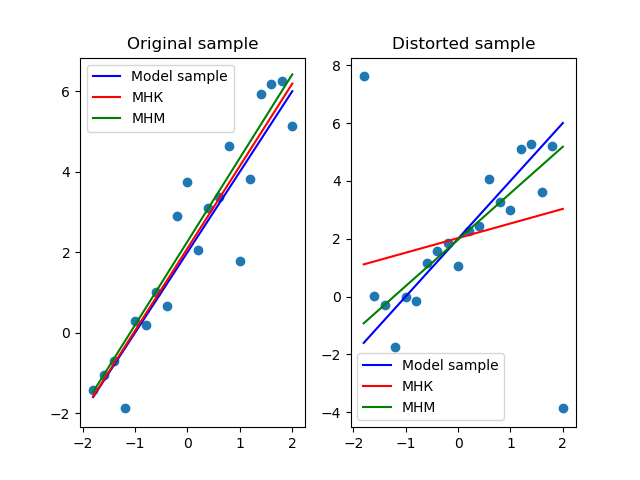
\includegraphics[scale = 0.8]{lab6/reg.png} 
    \label{fig:reg}
\end{figure}

\begin{table}[H]
\caption{Таблица оценок коэффициентов линейной регрессии без возмущёний}
\label{tab:my_label1}
\begin{center}
\vspace{5mm}
\begin{tabular}{|c|c|c|}
\hline
& $\overset{\wedge}{a}$ & $\overset{\wedge}{b}$\\
\hline
МНК &2.000&2.000\\
\hline
МНМ &1.926&2.372\\
\hline
\end{tabular}
\end{center}
\end{table}


\begin{table}[H]
\caption{Таблица оценок коэффициентов линейной регрессии с возмущёниями}
\label{tab:my_label2}
\begin{center}
\vspace{5mm}
\begin{tabular}{|c|c|c|}
\hline
& $\overset{\wedge}{a}$ & $\overset{\wedge}{b}$\\
\hline
МНК &2.000&2.000\\
\hline
МНМ &0.755 &1.938\\
\hline
\end{tabular}
\end{center}
\end{table}
% subsection оценка_линейной_регрессии (end)
\subsection{Метод максимального правдоподобия}

При подсчете оценок параметров закона нормального распределения методом максимального правдоподобия были получены следующие значения:
\begin{equation}
\begin{split}
    &\overset{\wedge}{m}_{\text{МП}} = -0.1235\\
   &  \overset{\wedge}{\sigma}^2_{\text{МП}} = 0.9877
\end{split}
\end{equation}
\subsection{Критерий Пирсона}
\begin{table}[H]
\caption{Таблица вычислений $\chi^2$}
\label{tab:my_label1}
\begin{center}
\vspace{5mm}
\begin{tabular}{|c|c|c|c|c|c|c|}
\hline
 i & $\Delta_i$ & $n_i$ & $p_i$ & $np_i$ & $n_i-np_i$ & $\frac{(n_i-np_i)^2}{np_i}$\\
\hline
1&	 $(-\infty, -1.8018]$ &	4  &	 0.0531	& 5.3136 &	 -1.3136 &	 0.3247\\
\hline
2&	(-1.8018, -0.4727)&	31&	 0.3025&	 30.2454&	 0.7546&	 0.0188\\
\hline
3& (-0.4727, 0.8564)&	47&	 0.4535&	 45.3525& 1.6475&	 0.0599\\
\hline
4&	$(0.8564, \infty)$&	18&	 0.1909&	 19.0886&	 -1.0886&	 0.0621\\
\hline
$\sum$&&		100&	1&	100&0&0.4655	\\

\hline
\end{tabular}
\end{center}
\end{table}

$$\chi_B^2= 0.4655$$

% subsection точечная_оценка_параметров_распределения (end)
\subsection{Интервальная оценка параметров распределения} % (fold)
\label{sub:интервальная_оценка_параметров_распределения}
\begin{table}[H]
\caption{Результаты интервальной оценки}
\label{tab:my_label1}
\begin{center}
\vspace{5mm}
\begin{tabular}{|c|c|c|c|}
\hline
Метод & $n$&$\mu$&$\sigma$\\
\hline
&$20$&	$[-0.60643, 0.16116]$&		$[0.73526, 1.41287]$ \\
\cline{2-4}
\raisebox{1.5ex}[0cm][0cm]{На основе ММП}&100&	$[-0.06206, 0.30951]$&		$[0.81800, 1.08155]$\\
\hline
&20&	$[-0.64667,0.20140]$&		$[0.68468, 1.25038]$ \\
\cline{2-4}
\raisebox{1.5ex}[0cm][0cm]{Асимптотический}&100	&$[-0.05888, 0.30633]$&	$[0.80817, 1.05515]$\\
\hline
\end{tabular}
\end{center}
\end{table}
\newpage
% subsection интервальная_оценка_параметров_распределения (end)
% section результаты (end)
\section{Выводы} % (fold)
\label{sec:выводы}
\subsection{Вычисление коэфицентов корреляции} % (fold)
\label{sub:вычисление_коэфицентов_корреляции}
При увеличении объёма выборки, подсчитанные коэффициенты корреляции стремятся к теоретическим. По графикам видно, что при уменьшении корреляции эллипс равновероятности стремится к окружности, а при увеличении растягивается.
\subsection{Оценки линий регрессии} % (fold)
\label{sub:оценки_линий_регрессии}
По графику \ref{fig:reg} видно, что оба метода дают хорошую оценку коэффициентов линейной регрессии, если нет выбросов. Так же видно, что выбросы больше влияют на оценку по МНК,
нежели на оценку по МНМ.
\subsection{Точечная оценка параметров распределения} % (fold)
\label{sub:точечная_оценка_параметров_распределения}
В данной работе получено значение критерия согласия Пирсона $\chi_B^2 = 0.4655$ Табличное значение квантиля  $\chi^2_{1-\alpha}(k-1)=\chi^2_{0.95}(4) = 9,4877$ \cite{chi_quant}.

Значит $\chi_B^2 < \chi^2_{0.95}(4),$ из этого следует, что основная гипотеза $H_0$ соотносится с выборкой на уровне $\alpha = 0.05.$
\subsection{Интервальная оценка параметров распределения} % (fold)
\label{sub:интервальная_оценка_параметров_распределения}
При увеличении объёма выборки точность увеличивается для обоих методов.
% subsection интервальная_оценка_параметров_распределения (end)
% subsection точечная_оценка_параметров_распределения (end)
% subsection оценки_линий_регрессии (end)
% subsection вычисление_коэфицентов_корреляции (end)
% section выводы (end)
\newpage
\begin{thebibliography}{}
    \bibitem{numpy}  Модуль numpy  -  https://physics.susu.ru/vorontsov/language/numpy.html
    
    \bibitem{plotlib} 
    Модуль matplotlib - https://matplotlib.org/users/index.html
    
    \bibitem{skp}
    Модуль scipy - https://docs.scipy.org/doc/scipy/reference/
    
\bibitem{lin_reg}
    https://en.wikipedia.org/wiki/Linear\_regression

\bibitem{8_1}
https://en.wikipedia.org/wiki/Confidence\_interval

\bibitem{8_2}
https://en.wikipedia.org/wiki/Student\%27s\_t-distribution

\bibitem{8_3}
https://en.wikipedia.org/wiki/Chi-squared\_distribution
\bibitem{chi_quant}
Таблица значений $\chi^2$ -  https://ru.wikipedia.org/wiki/\%D0\%9A\%D0\%B2\%D0\%B0\%D0\%BD\%D1\%82\%D0\%B8\%D0\%BB\%D0\%\do-B8\_\%D1\%80\%D0\%B0\%D1\%81\%D0\%BF\%D1\%80\%D0\%B5\%D0\%B4\%D0\%B5\%D0\%BB\%D0\%B5\%D0\%\do-BD\%D0\%B8\%D1\%8F\_\%D1\%85\%D0\%B8-\%D0\%BA\%D0\%B2\%D0\%B0\%D0\%B4\%D1\%80\%D0\%B0\%D1\%\do-82\%D0\%B2\%D0\%B0\%D0\%B4\%D1\%80\%D0\%B0\%D1\%82
\bibitem{8_4}
Шевляков Г. Л. Лекции по математической статистике, 2019.
    
\bibitem{mix}
    http://stu.sernam.ru/book\_stat3.php?id=55
    
\bibitem{5_1}
Двумерное нормальное распределение: https://en.wikipedia.org/wiki/Multivariate\_normal\_distribution
\bibitem{5_2}
Коэффициент корреляции Пирса: http://statistica.ru/theory/koeffitsient-korrelyatsii/ 
\bibitem{5_3}
Коэффициент корреляции Спирмана: 
http://economic-definition.com/Exchange\_Terminology/Koefficient\_korrelyacii\_Correlation\_coefficient\_\_eto.html
\bibitem{5_4} Квадрантный коэффициент корреляции: https://www.researchgate.net/profile/Pavel\_Smirnov8/publication/\do-316973167\_Robastnye\_metody\_i\_algoritmy\_ocenivania\_korrelacionnyh\_harakteristik\_dannyh\_na\_os\do-nove\_novyh\_vysokoeffektivnyh\_i\_bystryh\_robastnyh\_ocenok\_masstaba/links/591b019d458515695282\do-8a52/Robastnye-metody-i-algoritmy-ocenivania-korrelacionnyh-harakteristik-dannyh-na-osnove-novyh-vysokoeffektivnyh-i-bystryh-robastnyh-ocenok-masstaba.pdf\#page=81
\end{thebibliography}
\end{document}